% Options for packages loaded elsewhere
\PassOptionsToPackage{unicode}{hyperref}
\PassOptionsToPackage{hyphens}{url}
\PassOptionsToPackage{dvipsnames,svgnames,x11names}{xcolor}
%
\documentclass[journal=,manuscript=]{achemso}
\usepackage[version=3]{mhchem}
\newcommand*\mycommand[1]{\texttt{\emph{#1}}}



\usepackage{amsmath,amssymb}
\usepackage{iftex}
\ifPDFTeX
  \usepackage[T1]{fontenc}
  \usepackage[utf8]{inputenc}
  \usepackage{textcomp} % provide euro and other symbols
\else % if luatex or xetex
  \usepackage{unicode-math}
  \defaultfontfeatures{Scale=MatchLowercase}
  \defaultfontfeatures[\rmfamily]{Ligatures=TeX,Scale=1}
\fi
\usepackage{lmodern}
\ifPDFTeX\else  
    % xetex/luatex font selection
\fi
% Use upquote if available, for straight quotes in verbatim environments
\IfFileExists{upquote.sty}{\usepackage{upquote}}{}
\IfFileExists{microtype.sty}{% use microtype if available
  \usepackage[]{microtype}
  \UseMicrotypeSet[protrusion]{basicmath} % disable protrusion for tt fonts
}{}
\makeatletter
\@ifundefined{KOMAClassName}{% if non-KOMA class
  \IfFileExists{parskip.sty}{%
    \usepackage{parskip}
  }{% else
    \setlength{\parindent}{0pt}
    \setlength{\parskip}{6pt plus 2pt minus 1pt}}
}{% if KOMA class
  \KOMAoptions{parskip=half}}
\makeatother
\usepackage{xcolor}
\setlength{\emergencystretch}{3em} % prevent overfull lines
\setcounter{secnumdepth}{5}
% Make \paragraph and \subparagraph free-standing
\ifx\paragraph\undefined\else
  \let\oldparagraph\paragraph
  \renewcommand{\paragraph}[1]{\oldparagraph{#1}\mbox{}}
\fi
\ifx\subparagraph\undefined\else
  \let\oldsubparagraph\subparagraph
  \renewcommand{\subparagraph}[1]{\oldsubparagraph{#1}\mbox{}}
\fi


\providecommand{\tightlist}{%
  \setlength{\itemsep}{0pt}\setlength{\parskip}{0pt}}\usepackage{longtable,booktabs,array}
\usepackage{calc} % for calculating minipage widths
% Correct order of tables after \paragraph or \subparagraph
\usepackage{etoolbox}
\makeatletter
\patchcmd\longtable{\par}{\if@noskipsec\mbox{}\fi\par}{}{}
\makeatother
% Allow footnotes in longtable head/foot
\IfFileExists{footnotehyper.sty}{\usepackage{footnotehyper}}{\usepackage{footnote}}
\makesavenoteenv{longtable}
\usepackage{graphicx}
\makeatletter
\def\maxwidth{\ifdim\Gin@nat@width>\linewidth\linewidth\else\Gin@nat@width\fi}
\def\maxheight{\ifdim\Gin@nat@height>\textheight\textheight\else\Gin@nat@height\fi}
\makeatother
% Scale images if necessary, so that they will not overflow the page
% margins by default, and it is still possible to overwrite the defaults
% using explicit options in \includegraphics[width, height, ...]{}
\setkeys{Gin}{width=\maxwidth,height=\maxheight,keepaspectratio}
% Set default figure placement to htbp
\makeatletter
\def\fps@figure{htbp}
\makeatother

\usepackage{fontspec}
\setmainfont{Linux Libertine O}
\setsansfont{Linux Biolinum O}
\makeatletter
\@ifpackageloaded{caption}{}{\usepackage{caption}}
\AtBeginDocument{%
\ifdefined\contentsname
  \renewcommand*\contentsname{Table of contents}
\else
  \newcommand\contentsname{Table of contents}
\fi
\ifdefined\listfigurename
  \renewcommand*\listfigurename{List of Figures}
\else
  \newcommand\listfigurename{List of Figures}
\fi
\ifdefined\listtablename
  \renewcommand*\listtablename{List of Tables}
\else
  \newcommand\listtablename{List of Tables}
\fi
\ifdefined\figurename
  \renewcommand*\figurename{Figure}
\else
  \newcommand\figurename{Figure}
\fi
\ifdefined\tablename
  \renewcommand*\tablename{Table}
\else
  \newcommand\tablename{Table}
\fi
}
\@ifpackageloaded{float}{}{\usepackage{float}}
\floatstyle{ruled}
\@ifundefined{c@chapter}{\newfloat{codelisting}{h}{lop}}{\newfloat{codelisting}{h}{lop}[chapter]}
\floatname{codelisting}{Listing}
\newcommand*\listoflistings{\listof{codelisting}{List of Listings}}
\makeatother
\makeatletter
\makeatother
\makeatletter
\@ifpackageloaded{caption}{}{\usepackage{caption}}
\@ifpackageloaded{subcaption}{}{\usepackage{subcaption}}
\makeatother
\ifLuaTeX
  \usepackage{selnolig}  % disable illegal ligatures
\fi
\usepackage{bookmark}

\IfFileExists{xurl.sty}{\usepackage{xurl}}{} % add URL line breaks if available
\urlstyle{same} % disable monospaced font for URLs
\hypersetup{
  pdftitle={Functional complexity on cellular scale: Why in situ analyses are indispensable for our understanding of lignified tissues},
  pdfauthor={Leonard Blaschek; Henrik Serk; Edouard Pesquet},
  pdfkeywords={Lignin, In situ quantification, Cell
wall, Structure-function, Chemical imaging},
  colorlinks=true,
  linkcolor={blue},
  filecolor={Maroon},
  citecolor={Blue},
  urlcolor={Blue},
  pdfcreator={LaTeX via pandoc}}

\author{Leonard Blaschek}
\affiliation{ Copenhagen Plant Science Center (CPSC), Department of
Plant \& Environmental Sciences, University of Copenhagen,
Thorvaldsensvej 40, 1871 Frederiksberg C, Denmark,  }


\email{lb@plen.ku.dk}
\author{Henrik Serk}
\affiliation{ Umeå Plant Science Centre (UPSC), Department of Plant
Physiology, Umeå University, 901 87 Umeå, Sweden,  }


\author{Edouard Pesquet}
\affiliation{ Department of Ecology, Environment and Plant Sciences
(DEEP), Stockholm University, 106 91 Stockholm, Sweden,  }




\keywords{LigninIn situ quantificationCell
wallStructure-functionChemical imaging}

\title[]{Functional complexity on cellular scale: Why \emph{in situ}
analyses are indispensable for our understanding of lignified tissues}
\makeatletter
\begin{document}
\maketitle
\begin{abstract}
Lignins are a key adaptation enabling vascular plants to thrive in
terrestrial habitats. Lignin is heterogeneous -- containing upwards of
30 different monomers -- and its function multifarious: It provides
structural support, predetermined breaking points, UV-protection,
diffusion barriers, pathogen resistance and drought resilience. Recent
studies, carefully characterising lignin \emph{in situ,} have started to
identify specific lignin compositions and ultrastructures with distinct
cellular functions, but our understanding remains fractional. We
summarise recent works and highlight where further \emph{in situ} lignin
analysis could provide valuable insights into plant growth and
adaptation. We also summarise strengths and weaknesses of lignin
\emph{in situ} analysis methods.
\end{abstract}

\emph{Note: This manuscript was published behind a paywall in JAFC
(\href{https://doi.org/10.1021/acs.jafc.4c01999}{DOI:
10.1021/acs.jafc.4c01999}), as part of a special issue related to the
International Conference on Polyphenols 2023. The only difference
between this document\footnote{Additionally, the reproducible
  manuscript, including all R code to generate the figures, is available
  under
  \url{https://leonardblaschek.github.io/assets/2024_JAFC/index.html}.}
and the published version are the changes made by the ACS editorial
office. The American Chemical Society demanded \$4500 for making the
published version available to the public.}

\subsection{A versatile polymer}\label{a-versatile-polymer}

\emph{Lignin is the second-most abundant biopolymer on earth.} This
oft-repeated phrase urges us to understand the importance of this
complex phenolic polymer as a function of the sheer quantities present
in our biosphere. It is a very compelling framing, considering the
enormous potential of lignin as carbon sink and industrial resource from
ecological and economical perspectives respectively. From a
physiological point-of-view, however, focusing only on the abundance of
lignin -- or more precisely \emph{lignins,} as we are referring to
various, chemically distinct polymers -- risks overlooking its
impressive versatility with respect to cellular function. Tightly
delineated deposition of lignins, adapted in timing and composition to
various cell types and cell wall layers, is paramount for healthy plant
growth --- and their efficient use by us. It is worth contemplating,
then, whether \emph{where} lignin accumulates might be more important
than \emph{how much} of it there is overall.

\scriptsize


\begin{longtable}[]{@{}
  >{\raggedright\arraybackslash}p{(\columnwidth - 8\tabcolsep) * \real{0.1173}}
  >{\raggedright\arraybackslash}p{(\columnwidth - 8\tabcolsep) * \real{0.0510}}
  >{\raggedright\arraybackslash}p{(\columnwidth - 8\tabcolsep) * \real{0.2653}}
  >{\raggedright\arraybackslash}p{(\columnwidth - 8\tabcolsep) * \real{0.3929}}
  >{\raggedright\arraybackslash}p{(\columnwidth - 8\tabcolsep) * \real{0.1735}}@{}}

\caption{\label{tbl-locations}Diverse functions of lignins in plants.
Occurrence and regulation of several of the listed lignins are
summarized elsewhere;\citep{Chantreau2022} for detailed references, see
supplementary table S1. PCW -- primary cell wall; SCW -- secondary cell
wall. H/G/S refer to H (hydroxyphenyl), G (guaiacyl) and S (syringyl)
units in general, while H\textsubscript{CHOH}, G\textsubscript{CHOH},
G\textsubscript{CHO}, S\textsubscript{CHOH} and S\textsubscript{CHO}
specifically refer to \emph{p}-coumaryl alcohol, coniferyl alcohol,
coniferaldehyde, sinapyl alcohol and sinapaldehyde derived residues,
respectively.}

\tabularnewline

\toprule\noalign{}
\begin{minipage}[b]{\linewidth}\raggedright
Cell type
\end{minipage} & \begin{minipage}[b]{\linewidth}\raggedright
Wall type
\end{minipage} & \begin{minipage}[b]{\linewidth}\raggedright
Function
\end{minipage} & \begin{minipage}[b]{\linewidth}\raggedright
Lignin
\end{minipage} & \begin{minipage}[b]{\linewidth}\raggedright
Reference
\end{minipage} \\
\midrule\noalign{}
\endhead
\bottomrule\noalign{}
\endlastfoot
Abscission zones & PCW \& SCW & Focus external forces; restrict enzyme
diffusion & \emph{currently unknown} &
\citep{Lee2018, Balanza2016} \\
Bark and rind & SCW & Abiotic and biotic barrier & Over-representation
of atypical monomers (e.g.~flavonoids, hydroxystilbenes) &
\citep{Rencoret2019, Rencoret2022} \\
Casparian strip & PCW & Root diffusion barrier & Primarily
G/S\textsubscript{CHOH} and G/S\textsubscript{CHO} &
\citep{Reyt2021} \\
Compression wood & SCW & Support against gravity & Increased H &
\citep{Hiraide2021} \\
Endodermis cell corner & PCW & Compensation for Casparian strip defects
& More G\textsubscript{CHO} than the Casparian strip &
\citep{Reyt2021} \\
Exodermis & PCW & Root diffusion barrier & \emph{currently unknown} &
\citep{Manzano2022} \\
Endocarp & SCW & Fruit resilience, dispersal, water management &
\emph{currently unknown} &
\citep{Xiao2020, Huss2021} \\
Glandular trichome & PCW & Diffusion barrier increasing local Si
concentration & \emph{currently unknown} &
\citep{Hao2024} \\
Parenchyma & PCW & Restriction of pathogen/herbivore success & Increased
S; incorporation of feruloyltyramine &
\citep{Lee2019, Joo2021, Cesarino2019} \\
Pollen & SCW & Reinforces sporopollenin to maintain viability &
Primarily H\textsubscript{CHOH} &
\citep{Yang2023} \\
Replum & SCW & Pod shattering & \emph{currently unknown} &
\citep{Ballester2017} \\
Seed coat & SCW & Water management and biotic defense & Species-dep.
incorporation of caffeyl lingin &
\citep{Zhuo2022} \\
Stone cells & SCW & Damage insect mouth parts & Higher lignin conc. than
xylem &
\citep{Whitehill2016} \\
Tracheary elements & SCW & Balance stiffness, flexibility, waterproofing
& Primarily G\textsubscript{CHOH} and G\textsubscript{CHO} &
\citep{Menard2022, Blaschek2023} \\
Xylem fibres & SCW & Balance stiffness, flexibility, waterproofing &
Primarily G/S\textsubscript{CHOH} and G/S\textsubscript{CHO} &
\citep{Menard2022, Blaschek2023} \\
Xylem cell interface & PCW & Adjusts intercellular cohesion of vascular
tissues & Enriched in H; quantities vary between species &
\citep{Mottiar2020, Boyce2004} \\

\end{longtable}

\normalsize

\subsection{Plants tailor cell type-specific
lignins}\label{plants-tailor-cell-type-specific-lignins}

Lignins are formed by all vascular plants and in all plant organs. They
accumulate in the cell wall, a semi-crystalline composite of mainly
polysaccharides -- cellulose, hemicelluloses and pectins -- surrounding
the protoplast of each plant cell.\citep{Pedersen2023} Where exactly
these lignins accumulate, however, is controlled with nanometre
precision (Table~\ref{tbl-locations}). Fundamentally, lignification
requires two components: Oxidative enzymes and monomers. Laccases (LACs)
and peroxidases (PRXs) -- resilient, glycosylated phenoloxidases -- are
responsible for lignin polymerization.\citep{Blaschek2021} In lignifying
primary and secondary cell walls (PCWs and SCWs), LACs and PRXs are
expressed concomitantly with the enzymes responsible for biosynthesis of
cellulose and other cell wall polysaccharides.\citep{Blaschek2023} In
contrast to cellulose synthases or glucosyltransferases involved in
hemicellulose formation, LACs and PRXs are exported into the apoplast,
where they are embedded into the forming cell wall. Both types of
enzymes play important roles --- LACs are indispensable for xylem
lignification, while Casparian strip integrity depends on
PRXs.\citep{Blaschek2021, Blaschek2023, Rojas-Murcia2020} Paralogs of
both enzyme groups are immobilized in different cell types and cell wall
layers, enabling specific functions.\citep{Hoffmann2020, Blaschek2023}
Lignin monomers are a large group of phenolic compounds recently
summarized with great insight by John Ralph and
colleagues.\citep{Ralph2023} Most common and abundant are
phenylpropanoids with different ring substitutions, for example
4-hydroxyphenyl (H) units with a 4-hydroxyl, guaiacyl (G) units with an
additional 3-methoxy and syringyl (S) units with a further 5-methoxy. In
addition to their ring structures, these phenylpropanoid monomers also
vary in their aliphatic functional group, usually exhibiting an alcohol
(CHOH) or aldehyde (CHO). At the onset of cell wall lignification,
lignin monomers are exported from the cytosol into the cell wall. How
exactly this transport is catalyzed is also still contentious, with
recent evidence favoring a diffusion-based mechanism.\citep{Perkins2022}
Here, we should also note that it is not yet clear in which form lignin
monomers are exported and polymerized --- it might include unconjugated,
glycosylated or esterified phenolics. In the cell wall, lignin monomers
undergo 1-electron oxidation by LACs or PRXs, respectively using
O\textsubscript{2} or H\textsubscript{2}O\textsubscript{2} as electron
acceptor. The resulting radicals -- stabilised by mesomeric resonance
forms -- react either with each other to form dimers or extend a growing
polymer.\citep{Ralph2023} Depending on the involved monomers and
reaction environments, lignin polymerization generates a variety of
different --C--O--C and --C--C-- bonds resulting in structurally and
compositionally diverse polymers.\citep{Ralph2023} In the xylem, these
steps occur continuously and cell--cell cooperatively. Newly developing
tracheary elements -- the conduits of hydromineral sap -- undergo
programmed cell death before they lignify. The monomers for their
``post-mortem'' lignification are supplied by adjacent, still living
tracheary elements or (ray) parenchyma cells, or over longer distances
through the xylem sap.\citep{Pesquet2013, DeMeester2021, Zhang2020a}
This enables tracheary elements, and to a lesser extent fibers, to
continue adjusting their biomechanical and biophysical characteristics
long after they died.\citep{Menard2022} The resulting lignin composition
is partly a result of the monomers available during
polymerization.\citep{Ralph2023} Additionally, variations in substrate
specificity between LAC paralogs fine-tune lignin biochemistry on the
nanoscale.\citep{Blaschek2023, Zhuo2022} Lastly, dirigent proteins can
direct lignification to favor specific stereochemistries.\citep{Gao2023}
Together, these processes lead to a highly heterogeneous distribution of
specific lignins, which is largely conserved among vascular plants.
Angiosperm fibres, for example, have a higher S/G ratio and lower
G\textsubscript{CHO}/G\textsubscript{CHOH} ratio than tracheary
elements.\citep{Menard2022} For cell types outside of the xylem, this
type of lignin composition data is still exceedingly rare, although some
tendencies can be extracted from the literature
(Table~\ref{tbl-locations}).

Within cell walls, lignins fill out the spaces between cell wall
polysaccharides. Lignins interact non-covalently with both
hemicelluloses and cellulose,\citep{Kirui2022} and even form covalent
crosslinks with hemicelluloses and potentially
pectins.\citep{Giummarella2019} By reducing the water-accessible surface
areas of cell wall polysaccharides, lignins set the cell wall hydration
capacity and enable it to retain a quasi-constant volume irrespective of
the surrounding water availability.\citep{Blaschek2023} The prevalence
and effects of these interactions are distinct depending on species,
cell type and lignin biochemistry.\citep{Kirui2022} The cross-linking
and ``curing'' of cell walls by such interactions is likely a
significant aspect of lignin's various functions. To what extent the
monomeric composition and degree of cross-linking differs between cell
types responsible for water conduction and lateral distribution
(tracheary elements), biomechanical support (fibres), diffusion barriers
(endo-/exodermis), or pathogen defense (stress lignin), is only
beginning to be understood (Table~\ref{tbl-locations}).

\begin{figure}

\centering{

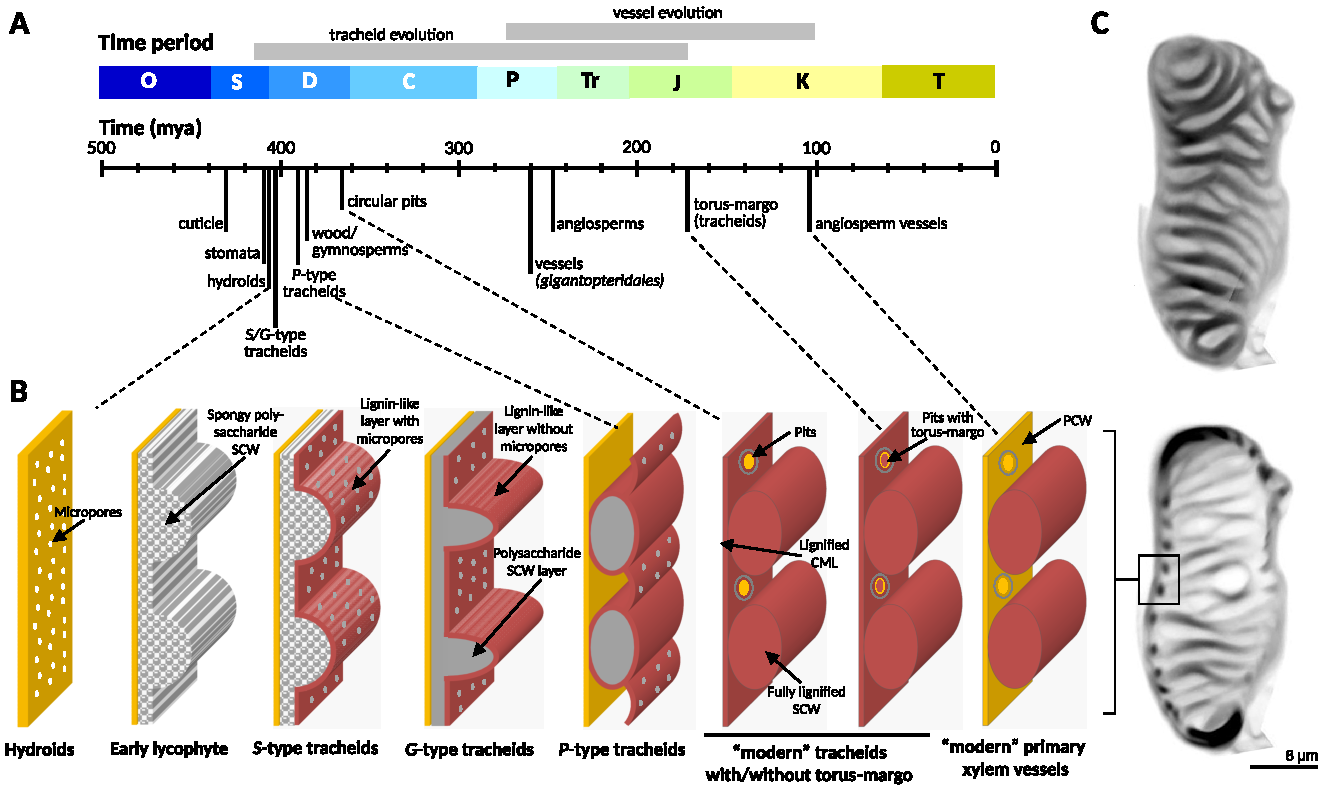
\includegraphics[width=1\textwidth,height=\textheight]{./data/evolution.pdf}

}

\caption{\label{fig-evolution}Schematic representation of tracheary
element sidewall modification during plant evolution and speciation. (A)
Main morphological changes in plants and tracheary elements during
evolution relatively to geological time with O -- Ordovician, S --
Silurian, D -- Devonian, C - Caboniferous, P - Permian, Tr - Triassic, J
- Jurassic, K - Cretaceous and T - Tiertary . (B) Evolutionary changes
of water-conducting cell sidewalls in terrestrial plants, SCW --
Secondary Cell Walls, PCW -- Primary cell walls, and CML -- compound
middle lamella. Red indicates lignin accumulation. Ancestral SCW
architectures are named \emph{Gosslingia} (G-type), \emph{Psilophyton}
(P-type) and \emph{Sennicaulis} (S-type), after the species in which
they were first described.\citep{Edwards2003} (C) Cell walls in a
tracheary element from inducible pluripotent suspension cell clultures
of the angiosperm \emph{Arabidopsis thaliana,} imaged by confocal laser
scanning microscopy of fluorescently stained cell wall polysaccharides.
Different optical sectioning provides a surface view (top) and a
cross-section (bottom). A portion of the cell wall equivalent to the
illustrations in panel B is highlighted.}

\end{figure}%

\subsection{The evolution of patterned
lignification}\label{the-evolution-of-patterned-lignification}

Analyses of fossil and extant plant sample collections reaching back to
the Devonian have been instrumental in showing the importance of the
spatial control of lignin accumulation for vascular plant evolution.
Around 410 million years ago, terrestrial bryophytes had developed the
initial blueprints of the tracheary element prototype: the hydroids --
cells forming water conducting tubes by undergoing programmed cell
death. Compared with water transport through plasmodesmata, the
development of hydroids improved water transport by more than
6-fold.\citep{Sperry2003} In some moss genera such as \emph{Sphagnum,}
hydroid lateral cell walls are reinforced by patterned SCWs to combine
lateral porosity in the gaps with mechanical reinforcement in rib-like,
lignin-free thickenings.\citep{Ligrone2000} Bryophytes are devoid of
lignins, but form other phenolic polymers like melanins and
coumaroyl-ester polymers in cuticles.\citep{Renault2017} The
evolutionary outburst of the Devonian saw the emergence of tracheary
elements. They proved considerably more efficient than hydroids due to
the addition of perforations for improved sap flow and lignified SCWs
for better mechanical support.\citep{Sperry2003} This evolutionary
enhancement in pro-vascular plants, such as observed in fossils of
\emph{Aglaophyton} and \emph{Hornephyton}, started with the formation of
micropores onto the pro-tracheary element sidewalls impregnated with
lignin-like polymers (Figure~\ref{fig-evolution}).\citep{Ligrone2000}
Next, both the layering and patterning of cell wall depositions changed,
with the first occurrence of banded/spiral SCW patterns in rhynopsid
fossils and named after \emph{Sennicaulis} (S-type pattern), resembling
modern protoxylem tracheary elements.\citep{Edwards2003} However, in
contrast to modern cells, the accumulation of lignin-like polymers in
S-type tracheary elements is uniformly covering the SCW luminal
surface.\citep{Edwards2003} This was followed by the emergence of
\emph{Gosslingia} (G-type) SCW patterns in lycophytes, maintaining the
banded/spiral motives but with larger micropores present in the gaps;
lignin-like polymers were still only present in a surface layer towards
the cell lumen.\citep{Edwards2003} S- and G-type lignin-like polymers
are considered the ancestral origin of lignins for all vascular plants.
Progressing through the Devonian, SCW pattern also diversified to
resemble modern metaxylem tracheary elements with reticulate/pitted
motives such as observed in \emph{Psilophyton} (P-type) tracheary
elements that developed pits interspersed in SCWs with a less uniform
lignin-like surface coverage depending on the cell wall
thickness.\citep{Edwards2003} Further evolutionary refinement first
enabled tracheary elements in gymnosperms to fully impregnate all cell
wall layers with lignin. Already then, lignin chemistry was specifically
delineated between cell wall layers, such as in the torus margo of its
lateral pits.\citep{Schulte2021} Modern vessels with larger diameter and
perforation plates at the end-walls of tracheary elements appeared by
the mid-Cretaceous such as in fossils of
Gigantopteridales.\citep{Sperry2003} These modern vessels included a
variation in SCW pattern together with lignin accumulation restricted to
its thickenings and absent from the gaps (Figure~\ref{fig-evolution}).
Fiber cell types, with all their variation from tracheiform to libriform
fibers,\citep{Sperry2003} derived from tracheary elements by reducing
the density of SCW gaps in their sidewalls, increasing cell wall
polysaccharide amounts but also differently controlling both lignin
amount and chemistry. Both fiber cell types -- together with the
characteristically high ratio and S- to G-units in their lignin -- have
been suggested to have convergently evolved several times, \emph{e.g} in
angiosperms and specific species of lycophytes such as
\emph{Selaginella.}\citep{Jin2007} The evolution of enzyme paralogs and
their neofunctionalisation have been key to the diversification of
lignin chemistry. To acquire S lignins, angiosperms duplicated
cytochrome P450 oxidoreductase genes into at least two paralogs
(cinnamate 4-hydroxylase and ferulate 5-hydroxylase in Arabidopsis),
whereas the lycophyte \emph{Selaginella} extended the substrate range of
its only cytochrome P450 oxidoreductase to catalyze both
reactions.\citep{Weng2010} Although lignin spatial chemistry and content
is mainly conserved between homologous cell types in vascular plant
species, further adaptive changes in lignin spatial distribution
occurred during speciation. These include a gradual reduction of the
lignin ratio between PCWs and SCWs in tracheary elements of gymnosperms
and angiosperms compared to ferns and lycophytes.\citep{Boyce2004}
Extreme cases include the absence of lignin from PCWs of xylem cells in
eastern leatherwood \emph{Dirca palustris,}\citep{Mottiar2020} or even a
complete absence of lignin in all cell wall layers of tracheary elements
in the monocotyledon eelgrass \emph{Zostera marina.}\citep{Pfeifer2022}
As with monomer biosynthesis, such tight spatial regulation of lignin
polymerization is partly driven by gene duplication and reduction. The
number of LAC paralogs ranges from 11 to 70 (0.039--0.192\% of all
genes) in terrestrial plants compared to only 3 to 7 (0.015--0.036\%) in
aquatic angiosperms.\citep{Blaschek2021, Simoes2020} Once accumulated,
lignin deposits cannot be removed by the plant. The timing of specific
spatial accumulation of lignin is therefore carefully regulated and
conserved between species: in tracheary elements of both gymnosperms and
angiosperms, lignin varying in chemistry and amounts are progressively
accumulated from the most external to the most internal cell wall
layers. Environmental constraints also affect the spatial distribution
of lignin in both in quantity and composition. Gravitropic stress in
gymnosperms, for example, leads to the cell wall layer-specific
over-accumulation of H-rich lignins,\citep{Hiraide2021} while biotic
stresses in angiosperms trigger accumulation of S-rich lignins
(Table~\ref{tbl-locations}). Lignin spatial distribution has thus been
extensively selected during plant evolution and speciation to enable
specific cell wall layers and cell types to change quantities and
chemistries of accumulated lignin to best adjust to developmental and
environmental constraints.

\subsection{Lignification patterns determine plant
growth}\label{lignification-patterns-determine-plant-growth}

Perhaps unsurprisingly, considering the evolutionary success and
physiological importance of lignins, efforts to generate plants with
cell walls more amenable to industrial exploitation by reducing lignin
amount or changing its composition usually result in stunted growth
phenotypes.\citep{DeMeester2018, DeMeester2020, Menard2022, Sulis2023}
Despite this common observation, overall lignin content in stems of
poplar (\emph{Populus} spp.; Figure~\ref{fig-correlation} A) and
Arabidopsis (Figure~\ref{fig-correlation} B) poorly predicts plant
growth. Indeed, we can understand the importance of lignin only when
considering it in its cellular context --- specifically in tracheary
elements. There, compromised lignification leads to weakened SCWs that
collapse inwards under the negative pressure driving sap transport --
known as an \emph{irregular xylem} (\emph{irx}) phenotype. This
phenotype leads to impaired sap transport, limiting vertical plant
growth together with the biomechanical weakening of the stem.
Underlining the importance of this particular lignin function, tracheary
element-specific lignin concentration explains more than half of the
observed variation in plant height (Figure~\ref{fig-correlation} C).
Beside crude concentration, both S/G and
G\textsubscript{CHO}/G\textsubscript{CHOH} ratios have decisive effects
on cell wall biomechanics and \emph{irx},\citep{Menard2022} as do other
cell wall polymers. The extent of \emph{irx} explains almost 90\% of
impaired plant growth in greenhouse conditions
(Figure~\ref{fig-correlation} D). Indeed, restoring full lignification
only in tracheary elements of hypolignified, dwarfed Arabidopsis and
poplar mutants conferred wild type-like growth --- even though total
lignin levels in the stems remained
reduced.\citep{DeMeester2018, DeMeester2021} Such genetic
complementation restrictively in tracheary elements confirms that all
lignin in all cell types does not have the same impact on plant growth.
The importance of fibres and their lignified SCWs for plant growth and
mechanics might well be larger than this data set suggests ---
especially under field conditions. To conclusively disentangle the
functional importances of these closely linked cell types and their
distinct lignins, we need carefully planned experiments linking \emph{in
situ} lignin quantification with plant growth in a comprehensive set of
species and mutants.

The biomechanics of whole stems -- including \emph{e.g} the flexibility
conferred by higher CHO/CHOH ratios -- can be extrapolated reasonably
well from single cells.\citep{Menard2022} To some extent, however,
tissue biomechanics are an emergent property arising from the interplay
between cell types and cell wall layers with contrasting
characteristics. The perhaps most compelling example of this is the
xylem of the eastern leatherwood mentioned above, which has been
suggested to owe its eponymous flexibility to the formation of lignified
SCWs interfacing with each other through lignin-free, flexible
PCWs.\citep{Mottiar2020} To understand these interaction effects in
biochemistry and function of lignins, we first need reliable data with
(sub-)cellular resolution.

\phantomsection\label{cell-fig-correlation}
\begin{figure}[H]

\centering{

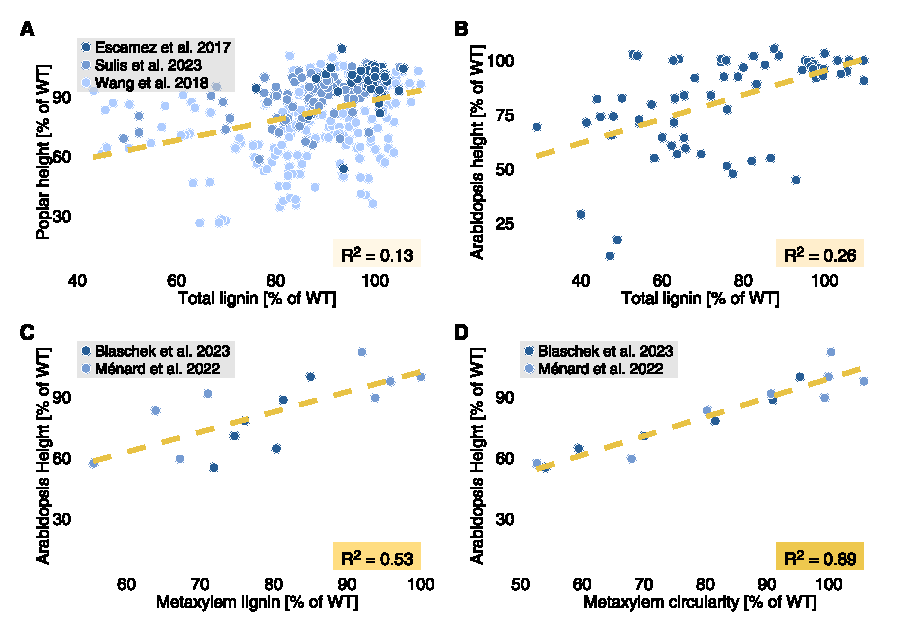
\includegraphics[width=1\textwidth,height=\textheight]{index_files/figure-pdf/fig-correlation-1.pdf}

}

\caption{\label{fig-correlation}Total lignin content is a poor predictor
of plant growth, while cell type-specific differences in lignin
concentration and their consequences -- in this case vessel collapse in
the metaxylem -- explain a much larger fraction of the observed variance
in plant height. Note that data containing cell-specific lignin
quantities -- and with it the conclusions we can draw from these
correlations -- are still sparse. Coefficients of determination for the
corresponding linear regression are indicated in each panel
(\emph{P}-values all \textless{} 0.05). For the collated data and
corresponding references see supplementary table S1.}

\end{figure}%

\subsection{\texorpdfstring{Methods for lignin \emph{in situ}
analysis}{Methods for lignin in situ analysis}}\label{methods-for-lignin-in-situ-analysis}

The complexity of lignin makes its biochemical analysis challenging.
Lignin monomeric composition is so diverse, and its association with
other cell wall polymers and hydrophobic extractives so tight, that
measuring \emph{all} lignins and \emph{only} lignins in a sample is near
impossible. Most traditionally used lignin analysis methods -- Klason,
acetyl bromide and thioglycolic acid assays among many others -- proceed
via sample milling and extraction to purify the majority of lignin.
While these methods estimate lignin concentration reasonably well, they
all have extensively debated biases\citep{Hatfield2005} and, crucially,
cannot provide detailed information about the cellular distribution of
lignin. The latter limitation can be mitigated, but not avoided, by
meticulous sampling by \emph{e.g.} laser micro dissection. The
alternative to extract-and-quantify methods is the \emph{in situ}
characterization of lignin. \emph{In situ} chemical imaging methods such
as the chromogenic Wiesner test or observation of lignin
autofluorescence have been used to detect lignin since the 19th century.
However, extracting reliable quantitative read-outs from such methods
has only become feasible in recent years, with improving instrumentation
and careful biochemical validation of the results. Conceptually, we can
describe methods for lignin \emph{in situ} analysis on three axes:
spatial resolution, chemical resolution and quantitative capacity
(Figure~\ref{fig-methods}). All methods represent trade-offs along these
three axes, with further differences in required effort and
instrumentation, which we roughly outline in the following (further
details of the mentioned methods and others are tabulated in the table
S1). Which of these methods will provide the most valuable insights
depends on the scientific question, and should be considered carefully.

\phantomsection\label{cell-fig-methods}
\begin{figure}[H]

\centering{

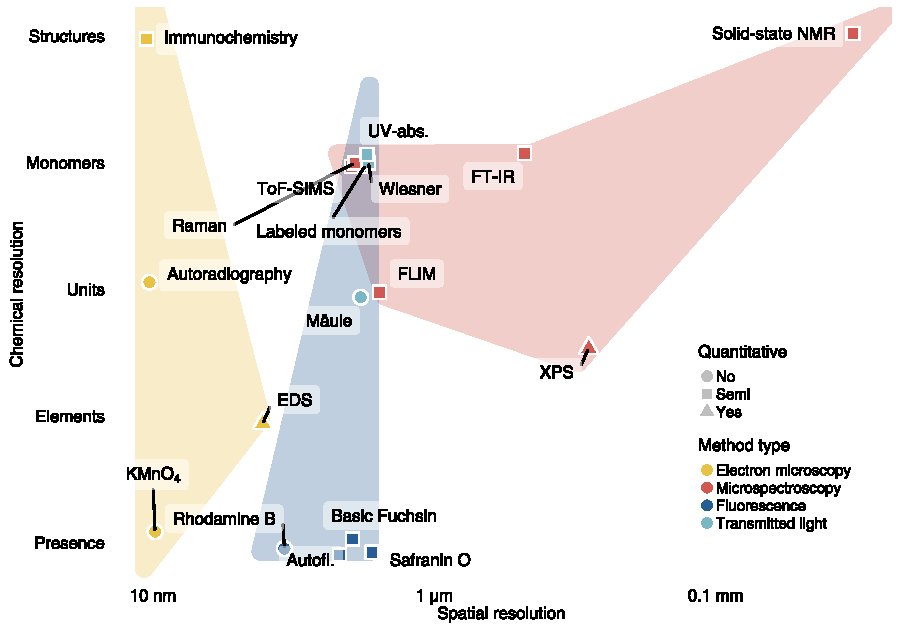
\includegraphics[width=1\textwidth,height=\textheight]{index_files/figure-pdf/fig-methods-1.pdf}

}

\caption{\label{fig-methods}Methods for \emph{in situ} lignin analysis.
Chemical and spatial resolution are estimates from what has been
validated and published, not what is theoretically possible. Note that
the distinction between microscopy and spectroscopy is arbitrary to some
extent --- here we drew the line based on the need for specialist
spectroscopic instrumentation. `Unit' refers to lignin ring structures
(\emph{e.g.} G), `monomers' to whole building blocks (\emph{e.g.}
G\textsubscript{CHO}), and `structures' to specific inter-monomeric
linkages. For the collated data and corresponding references see
supplementary table S1.}

\end{figure}%

\subsubsection{Electron microscopy}\label{electron-microscopy}

Electron microscopy in combination with the KMnO\textsubscript{4} lignin
stain, antibodies, or radioactively labelled precursors, provides
information about lignin distribution with the highest spatial
resolution. Those methods, depending on their sophistication, can also
yield very high chemical resolution (Figure~\ref{fig-methods}). Detailed
insight in the diversity of lignin polymers between cell wall layers was
shown using KMnO\textsubscript{4} staining to reveal a globular topology
in PCW layers compared to rod-shaped in SCWs, conserved between plant
species.\citep{Donaldson2001} Total sample size for electron microscopy
is limited, precluding full organ biopsies. However, the main weakness
of electron microscopy-based methods are the limited quantitative
read-outs. Although changes in radioactivity correlate with the
incorporation of radioactive precursors, both the possible
metabolisation of the fed compounds into chemically distinct monomers as
well as artefactual labeling due to mislocalisation of the compound
during feeding hinder any reliable semi-quantitative measurements. In
contrast, antibody density detected through gold particles correlates
more robustly with antigen density and several reports showed similar
semi-quantitative trends between cell wall layers, cell types and plant
species.\citep{Joseleau2004, Ruel2009} Nonetheless, both antibody
affinity and epitope accessibility can be hard to predict \emph{in
situ,} warranting careful interpretation. Very useful exceptions to this
quantitative limitation are X-ray microscopy and energy-dispersive X-ray
spectroscopy (EDS). X-ray microscopy can quantify aromatic carbons due
to their specific absorption to define lignin
distribution.\citep{Boyce2004} Similarly, EDS can be coupled with
electron microscopy to quantitatively map elemental abundances in the
sample --- albeit in practice with a slightly lower spatial resolution
than electron microscopy itself. Considering the much higher C/O ratio
of lignin compared to cell wall polysaccharides, EDS can estimate
relative lignin content with nanometre-precision.\citep{Menard2022}

\subsubsection{Micropscopy of transmitted light and
fluorescence}\label{micropscopy-of-transmitted-light-and-fluorescence}

Light microscopy methods, using chromogenic and fluorescent stains or
exploiting lignin autofluorescence, can provide semi-quantitative
read-outs with considerable spatial and chemical resolution. Given
adequate sample preparation, the spatial resolution of these methods is
close to the diffraction limit. The combination of fluorescent lignin
stains such as Rhodamine B with super-resolution microscopy even goes
beyond that, resolving differences in lignin quantity below 100
nm.\citep{Donaldson2022} Of the numerous chromogenic and fluorescent
lignin stains only very few have been validated regarding their
quantitative capacity and chemical specificity. The absorbance of the
Wiesner test represents a reliable way to estimate cell wall
layer-specific G\textsubscript{CHO} concentration \emph{in
situ.}\citep{Blaschek2020a} The Mäule test identifies cell walls rich in
S-units with a red hue, but whether it provides quantitative information
is yet to be determined.\citep{Yamashita2016} Safranin O fluorescence
emission ratios were suggested to be indicative of total lignin
concentration.\citep{Baldacci-Cresp2020} Considering the stark
disagreement between \emph{in situ} lignin estimates from Safranin O and
Raman measurements, however, it remains uncertain whether Safranin O
estimates total lignin or only a specific
fraction.\citep{Blaschek2023, Baldacci-Cresp2020} Basic Fuchsin,
Acriflavin and Auramine O all appear to represent trade-offs between
sensitivity and specificity that have yet to be biochemically
validated.\citep{Ursache2018} Lignin UV-autofluorescence and absorbance
also provide quantitative information. Total autofluorescence intensity
is considered to reflect total lignin concentration, although the
various observed spectral components are not definitively assigned to
specific lignin structures.\citep{Decou2019} The multimodal nature of
lignin autofluorescence extends to its lifetime, which has been
correlated to S/G ratios \emph{in situ,}\citep{Escamez2021} and likely
contains more, yet to be deciphered information about lignin chemistry.
The distinct UV-absorbance profiles of lignin monomers on the other hand
have been used to quantify S/G and
G\textsubscript{CHO}/G\textsubscript{CHOH} ratios \emph{in
situ.}\citep{Peng1997, Yoshida2005} Fluorescently-labeled lignin
monomers can either be directly conjugated to a fluorescent molecule or
decorated with a reactive group for subsequent \emph{in vivo} click
chemistry. Their distribution \emph{in situ} indicates where different
lignin monomers might be actively incorporated into lignin at the time
of feeding. The caveat is that the position of the fluorescent label or
click ligation site affects metabolization and polymerization of the fed
compounds. While these data give no direct information of lignin
quantity or composition, the method has been successfully used to for
example demonstrate LAC substrate-specificity in compression wood
lignification.\citep{Hiraide2021} Altogether, transmitted light and
fluorescence microscopy-based methods provide a useful, low-cost toolbox
for lignin characterisation \emph{in situ}. Moreover, and despite their
long history of use, neither lignin autofluorescence nor most lignin
stains are fully understood regarding their chemical specificities,
leaving much room for future improvements and discoveries.

\subsubsection{Microspectroscopy}\label{microspectroscopy}

Microspectroscopy read-outs have the highest information density. These
methods are generally label-free, exploiting inherent physicochemical
characteristics of the lignin polymers. Beside spectroscopic methods
based on fluorescence (discussed above), Raman and Fourier-transform
infrared (FT-IR) microspectroscopy are perhaps most commonly used for
lignin \emph{in situ} analysis. Both methods exploit the vibrational
states of covalent bonds --- Raman instruments detect photons scattered
by these shifting vibrational states, whereas FT-IR measures their
absorbance. Each bond creates a specific signal, which is further
modulated by the directly adjacent bonds. For lignin, that means that
the signal is influenced by the incorporated monomers, their position in
the polymer and the inter-molecular linkages.\citep{Yamamoto2020a}
Although they exploit the same physical phenomenon, Raman and FT-IR have
distinct advantages for cell wall analysis. FT-IR is more sensitive to
polar groups (O---H, C=O) and tends to provide less noisy spectra for
cell walls.\citep{Guillon2022} In return, the method is inherently
limited to resolutions in the µm range, requires very thin sections and
struggles with hydrated samples due to water
absorbance.\citep{Guillon2022} Raman on the other hand is more sensitive
to carbon bonds (C---C, C=C), allows spatial resolutions around 300 nm
and is insensitive to water in the sample.\citep{Guillon2022} It does
not require thin sections and can be used non-destructively on
\emph{e.g.} fossils.\citep{Qu2019} The downside of Raman
microspectroscopy is the enormous amount of spectral information
contained in each cell wall spectrum. Even more so than in FT-IR, the
numerous bonds in the sample result in a highly convoluted spectrum,
making the quantification of isolated bands difficult. One approach to
overcome this convolution is the unmixing of hypothetical ``pure''
molecules of different polymers in the sample, so-called endmembers.
Such unmixing has facilitated \emph{e.g.} the discovery that
hydrolyzable tannins are incorporated into the lignified cell walls of
\emph{Trapa natans} seeds.\citep{Huss2024} While useful, the large
effects of chosen algorithm and endmember number warrant careful
interpretation and validation of the unmixed spectra. Alternatively,
avoiding any potential artifacts of unmixing, spectra can be evaluated
without deconvolution. Although the precision of measurements acquired
with this approach is diminished by overlapping bands, it has been
successfully used to reveal lignin composition differences resulting
from distinct LAC
substrate-specificities.\citep{Blaschek2020, Blaschek2023} \emph{In
vitro,} isolated from the convoluted signal of plant cell walls, model
compounds of lignin monomers, oligomers (such as dibenzodioxocin) and
polymers can be distinguished in even more
detail.\citep{Bock2020, Blaschek2020}

Time-of-flight secondary ion mass spectrometry (TOF-SIMS) functions via
the ionization of molecules at the sample surface and their subsequent
mass-spectrometric identification. With an axial resolution of 1--2 nm,
lateral resolutions down to 50 nm and the capacity to in principle
distinguish any ionizable molecule, TOF-SIMS -- in theory -- trumps most
other methods for \emph{in situ} lignin analysis. In practice however,
used pixel sizes of range between 300 and 500 nm and the number of
empirically assigned peaks is limited, resulting lower resolutions and
signal-to-noise ratios than can be achieved with, for example, Raman
imaging. Additionally, the necessary sample drying can distort cell wall
layer organization. Nonetheless, TOF-SIMS offers unique opportunities
--- quantitative \emph{in situ} distinction of \emph{p}-hydroxybenzoate-
and S-units, for example, is not currently possible with any other
method.\citep{Mottiar2023}

X-ray photoelectron spectroscopy (XPS) and solid-state nuclear magnetic
resonance (NMR) spectroscopy are included here, in a collection of
\emph{in situ} imaging techniques, prospectively. XPS is routinely used
in cell wall analysis, providing absolute quantities of atoms and bonds
on the sample surface.\citep{Watts2022} Similarly, solid-state NMR is an
established technique that has provided some of the most exciting
insights into lignin--carbohydrate interactions in plant cell
walls.\citep{Kirui2022} In current practice, however, both of these
methods lack imaging features. XPS classically returns data from the
irradiated spot with a resolution around 10 µm, while NMR averages over
the entire, usually mm-sized sample. While not yet in common use for
biological samples, both single cell NMR and XPS imaging are feasible
and have seen rapid developments in recent years. If those developments
continue, XPS and NMR imaging might soon provide detailed sub-micron
information about elemental bonds and whole lignin structures
respectively.

\subsection{Concluding remarks}\label{concluding-remarks}

In the last three years, the methods outlined herein have been used to
dramatically alter our understanding of lignification. Until very
recently, the prevalent model considered that lignification was
exclusively controlled by monomer availability. Now we know that both
LAC/PRX substrate-specificity\citep{Blaschek2023, Hiraide2021, Zhuo2022}
and the molecular chaperoning by dirigent proteins\citep{Gao2023} have
decisive, cell type-specific effects on lignin amount and composition.
These mechanisms, along with monomer supply and LAC/PRX co-substrate
availability, direct a tightly regulated program of lignification,
leading to distinct sub-cellular localisations and compositions
depending on cell type, developmental status and environmental cues. For
most lignified cell types, however, we still have almost no data
capturing their lignin biochemistry with subcellular resolution. That
kind of data, combined with \emph{in situ} methods to probe cell wall
biomechanics and topology, will be crucial to understand which
structural aspects of lignified cell walls allow them to fulfill their
varying functions. It might seem like a purely fundamental research
question, but knowing how and where to modify lignins without impeding
plant growth or survival will be key to generate new, more efficient
feedstock for industrial exploitation. Hence, a detailed understanding
of lignin's cell type-specific structure-function relationships has the
potential to significantly advance our path to a sustainable economy.

\subsection{Acknowledgements}\label{acknowledgements}

We would like to thank the Groupe Polyphenols for the invitation to
contribute to this special issue. We also want to apologize to all the
colleagues whose excellent work we could not cite here due to space
constraints.

\subsection{Funding}\label{funding}

LB is supported by EMBO postdoctoral fellowship ALTF 37-2022. EP is
funded by Swedish Research council (Vetenskapsrådet VR) 2023-03661 and
Carl Tryggers Stiftelse CTS 23:2756.

\subsection{Data Availability}\label{data-availability}

All literature data collated for figures and tables can be found in
\href{https://pubs.acs.org/doi/suppl/10.1021/acs.jafc.4c01999/suppl_file/jf4c01999_si_001.xlsx}{supplementary
table S1 (link to ACS)}.

\subsection*{References}\label{references}
\addcontentsline{toc}{subsection}{References}

\renewcommand{\bibsection}{}
\bibliography{Zotero_lib_bibtex.bib}




\end{document}
